%  -*- mode: latex; coding: utf-8 -*-
%\documentclass{ltjsarticle}
\documentclass[b5]{ltjsbook}

\usepackage{xparse}
\usepackage[unicode=true]{hyperref}

% https://github.com/jperon/lyluatex/blob/master/README.md
\usepackage{lyluatex}

\usepackage{tikz}
\usetikzlibrary{arrows.meta,shapes,calc}
\usetikzlibrary{decorations.pathmorphing,decorations.pathreplacing, decorations.shapes}
%\usepackage{pgfplots}
\usepackage{latexsym}
\usepackage{amssymb}
\usepackage{lilyglyphs}
\newcommand{\bra}[1]{\left\langle#1\right|}
\newcommand{\ket}[1]{\left|#1\right\rangle}

\newcommand{\SeptimalSharp}{\includegraphics[height=0.8em]{images-svg/Heji38.png}}
\newcommand{\SeptimalFlat}{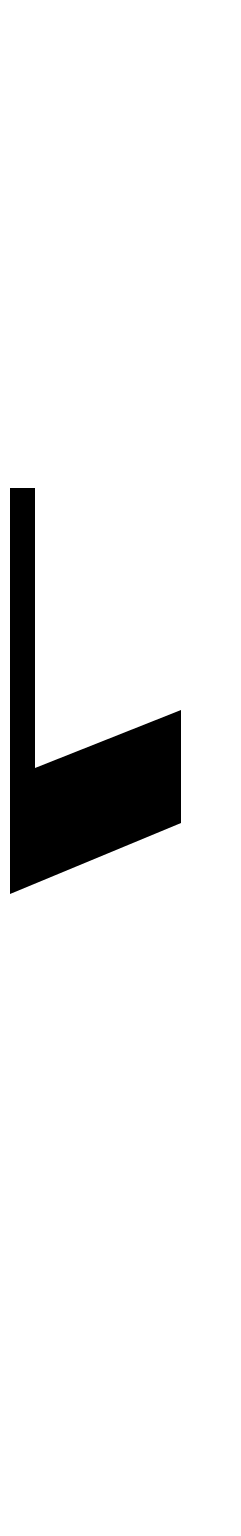
\includegraphics[height=0.8em]{images-svg/Heji37.png}}
%\newcommand{\SeptimalSharp}{+7}
%\newcommand{\SeptimalFlat}{-7}

%\usepackage[sourcehan]{luatexja-preset}
\usepackage{luatexja-preset}


\usepackage{amsmath}
\usepackage{nicefrac}

\setmainfont[Ligatures=TeX]{TeXGyreTermes}
\setsansfont[Ligatures=TeX]{TeXGyreHeros}
\setmonofont[Ligatures=TeX]{TeXGyreCursor}

\begin{lysavefrag}{clairnote}
\include "LilyPond-Clairnote/clairnote.ly"
\end{lysavefrag}
\lynewenvironment{lilypondClairnote}[1][]{%
  \begin{lilypond}[include_header={clairnote},#1]%
}{%
  \end{lilypond}%
}

\begin{document}

\title{代替記譜法のススメ}
\author{酒本典明}
\date{2025年1月17日}
\maketitle

\tableofcontents
\clearpage

\chapter{序文}
本書では代替記法

\part{Clairnoteのススメ}
\chapter{伝統記譜法の歴史}
\chapter{代替記譜法}
\chapter{Clairnote}
\chapter{Clairnote改善案}


\begin{lilypondClairnote}
<<
  \relative
  {
    \clef treble
    \key f \major
    \time 2/4

    c''8. d16 c8. d16 | c4 a8 r |
    a8. bes16 a8. bes16 | a4 f8 r |
  }
  \addlyrics
  {
    ゆ "" き や こん こ
    あ ら れ や こん こ
  }
>>
\end{lilypondClairnote}


\chapter{円形和音表記法}
\newcommand{\newJIAngle}[2]{\pgfmathsetmacro#1{360*ln(#2)/ln(2))}}
\newJIAngle{\jiIII}{3}
\newJIAngle{\jiV}{5}
\newJIAngle{\jiVII}{7}
\newJIAngle{\jiXI}{11}
\newJIAngle{\jiXIII}{13}
\newJIAngle{\jiXVII}{17}
\newJIAngle{\jiXIV}{19}
\newcommand{\drawJI}[3][]{%
  \pgfmathsetmacro{\startAngle}{90-(#2)}
  \pgfmathsetmacro{\endAngle}{(\startAngle)-(#3)}
  \draw[thick,#1] (\startAngle:\ccRadius) -- (\endAngle:\ccRadius);
}
\NewDocumentCommand\drawCircle{m}{
  \pgfkeysgetvalue{/chord circle/radius}{\ccRadius}

  % Draw the unit circle
  \draw[thick] (0,0) circle (\ccRadius);

  % Draw the notches
  \foreach \i in {0, 1, ..., 11} {
      \pgfmathsetmacro{\angle}{90-30*\i}
      \draw (\angle:{0.95*\ccRadius}) -- (\angle:{1.05*\ccRadius});
  }
}

\NewDocumentCommand\drawLabel{m m}{
  \pgfkeysgetvalue{/chord circle/radius}{\ccRadius}

  \pgfmathsetmacro{\angle}{90-(#1)}
  \pgfmathsetmacro{\anchor}{180+\angle}
  %\draw[thick] (\angle:{0.95*\ccRadius}) -- (\angle:{1.05*\ccRadius});
  \node[anchor=\anchor,align=center] at (\angle:{1.1*\ccRadius}) {#2};
}
\NewDocumentCommand\drawTickerBass{O{} m}{
  \pgfkeysgetvalue{/chord circle/radius}{\ccRadius}
  \pgfmathsetmacro{\angle}{90-(#2)}

  \node[rotate={\angle-90},align=center,inner sep=0pt] at
  (\angle:{1.07*\ccRadius}) {\scriptsize\textsf{-}};
}
\tikzset{cross/.style={cross out, draw=black, fill=none, minimum size=2*(#1-\pgflinewidth), inner sep=0pt, outer sep=0pt}, cross/.default={2pt}}
\NewDocumentCommand{\drawOmitted}{m}{
  \pgfkeysgetvalue{/chord circle/radius}{\ccRadius}
  \pgfmathsetmacro{\angle}{90-(#1)}
  \node[thick,cross,rotate={\angle}] at (\angle:{1.07*\ccRadius}) {};
}
\NewDocumentCommand\drawTicker{m}{
  \pgfkeysgetvalue{/chord circle/radius}{\ccRadius}

  \pgfmathsetmacro{\angle}{90-(#1)}
  \draw[thick] (\angle:{\ccRadius}) -- (\angle:{1.05*\ccRadius});
}
\NewDocumentCommand\drawIndicator{m}{
  \pgfkeysgetvalue{/chord circle/radius}{\ccRadius}

  \pgfmathsetmacro{\angle}{90-(#1)}
  \draw[thick] (\angle:{0.95*\ccRadius}) -- (\angle:{1*\ccRadius})
      node[draw,isosceles triangle,anchor=apex,rotate={\angle-180},minimum size=0.05*\ccRadius,inner sep=0pt]{};
}
\NewDocumentCommand{\drawNote}{O{ticker,label} m m}{%
  \pgfkeysdef{/chord circle/draw note/omitted}{\drawOmitted{#2}}
  \pgfkeysdef{/chord circle/draw note/ticker}{\drawTicker{#2}}
  \pgfkeysdef{/chord circle/draw note/indicator}{\drawIndicator{#2}}
  \pgfkeysdef{/chord circle/draw note/label}{\drawLabel{#2}{#3}}
  \pgfkeys{/chord circle/draw note/.cd,#1}
}
\NewDocumentCommand{\drawIntervalJI}{O{} O{} m m}{%
  \pgfkeysgetvalue{/chord circle/radius}{\ccRadius}

  \pgfmathsetmacro{\startAngle}{90-(#3)}
  \pgfmathsetmacro{\endAngle}{(\startAngle)-(#4)}
  \draw[thick,#1] (\startAngle:\ccRadius) -- (\endAngle:\ccRadius) #2;
}
\pgfkeyssetvalue{/chord circle/interval/JI/3/style}{-Stealth}
\NewDocumentCommand{\drawIntervalIII}{O{} m}{%
  \pgfkeysgetvalue{/chord circle/interval/JI/3/style}{\nodeStyle}
  \expandafter\drawIntervalJI\expandafter[\nodeStyle,#1]{#2}{\jiIII}
}
\pgfkeyssetvalue{/chord circle/interval/JI/5/style}{arrows={->[scale length=2]},dashed,red}
\NewDocumentCommand{\drawIntervalV}{O{} m}{%
  \pgfkeysgetvalue{/chord circle/interval/JI/5/style}{\nodeStyle}
  \expandafter\drawIntervalJI\expandafter[\nodeStyle,#1]{#2}{\jiV}
}
\pgfkeyssetvalue{/chord circle/interval/JI/7/style}{arrows={->[scale length=3]},decorate,decoration={saw},blue}
\NewDocumentCommand{\drawIntervalVII}{O{} m}{%
  \pgfkeysgetvalue{/chord circle/interval/JI/7/style}{\nodeStyle}
  \expandafter\drawIntervalJI\expandafter[\nodeStyle,#1]{#2}{\jiVII}
}
\NewDocumentCommand{\nodeCaption}{O{} m}{%
  \pgfkeysgetvalue{/chord circle/radius}{\ccRadius}

  \node[#1] at (-90:{1.5 * \ccRadius}) {#2};
}
\makeatletter
\newcommand\mathcircled[1]{%
  \mathpalette\@mathcircled{#1}%
}
\newcommand\@mathcircled[2]{%
  \tikz[baseline=(math.base)] \node[draw,circle,inner sep=1pt] (math) {$\m@th#1#2$};%
}
\makeatother


本節では著者考案の円形和音表記法について記す。

\begin{tikzpicture}
    \pgfkeyssetvalue{/chord circle/radius}{3cm}
    \drawCircle{}
    % Add axes
    %\draw[->] (-3.5, 0) -- (3.5, 0) node[right] {$x$};
    %\draw[->] (0, -3.5) -- (0, 3.5) node[above] {$y$};

    % Define the logarithm values and plot points

    \drawNote[indicator,label]{0}{$2=2^1\equiv\ket{0}$}
    \drawNote{30}{$2^{\frac{1}{12}}\equiv\ket{\nicefrac{1}{12};}$}
    \drawNote{60}{$2^{\frac{2}{12}}\equiv\ket{\nicefrac{2}{12};}$}
    \drawNote{90}{$2^{\frac{3}{12}}\equiv\ket{\nicefrac{3}{12};}$}
    \drawNote{120}{$2^{\frac{4}{12}}\equiv\ket{\nicefrac{4}{12};}$}
    \drawNote{150}{$2^{\frac{5}{12}}\equiv\ket{\nicefrac{5}{12};}$}
    \drawNote{180}{$2^{\frac{6}{12}}\equiv\ket{\nicefrac{6}{12};}$}
    \drawNote{210}{$2^{\frac{7}{12}}\equiv\ket{\nicefrac{7}{12};}$}
    \drawNote{240}{$2^{\frac{8}{12}}\equiv\ket{\nicefrac{8}{12};}$}
    \drawNote{270}{$2^{\frac{9}{12}}\equiv\ket{\nicefrac{9}{12};}$}
    \drawNote{300}{$2^{\frac{10}{12}}\equiv\ket{\nicefrac{10}{12};}$}
    \drawNote{330}{$2^{\frac{11}{12}}\equiv\ket{\nicefrac{11}{12};}$}

    \bgroup
    \pgfkeysgetvalue{/chord circle/radius}{\ccRadius}

    \draw[thick] (0,0) -- (0:\ccRadius);
    \draw[thick] (0,0) -- (30:\ccRadius);
    \draw[thick] (0,0) -- (60:\ccRadius);
    \draw[thick] (0,0) -- (90:\ccRadius);
    \draw[thick] (0,0) -- (120:\ccRadius);
    \draw[thick] (0,0) -- (150:\ccRadius);
    \draw[thick] (0,0) -- (180:\ccRadius);
    \draw[thick] (0,0) -- (210:\ccRadius);
    \draw[thick] (0,0) -- (240:\ccRadius);
    \draw[thick] (0,0) -- (270:\ccRadius);
    \draw[thick] (0,0) -- (300:\ccRadius);
    \draw[thick] (0,0) -- (330:\ccRadius);

    \node at (15:0.2*\ccRadius) {$\cdot$};
    \node at (45:0.2*\ccRadius) {$\cdot$};
    \node at (75:0.2*\ccRadius) {$\cdot$};
    \node at (105:0.2*\ccRadius) {$\cdot$};
    \node at (135:0.2*\ccRadius) {$\cdot$};
    \node at (165:0.2*\ccRadius) {$\cdot$};
    \node at (195:0.2*\ccRadius) {$\cdot$};
    \node at (225:0.2*\ccRadius) {$\cdot$};
    \node at (255:0.2*\ccRadius) {$\cdot$};
    \node at (285:0.2*\ccRadius) {$\cdot$};
    \node at (315:0.2*\ccRadius) {$\cdot$};
    \node at (345:0.2*\ccRadius) {$\cdot$};
    \egroup

    \nodeCaption[align=center]{12平均律};
\end{tikzpicture}

以下の要素からなる。
\begin{description}
\item[円周] 音高を示す目安となる。一周で周波数が2倍になる。つまり、1オクターブが一周である。
  時計周り方向に音が高くなる。9時方向をAとする。
\item[目安] 円周の内と外側に跨って描かれる。円周を12等分した音高を示す。
\item[音標] 円周の外側に描かれる。音高とそれに付随する要素を示す。
\item[浮標] 円周の外側、音標の近くに描かれる。音標の示す音に関係する情報を示す。
\item[音程] 円周の内に描かれる。音標の間の音程を示す。
\end{description}

音標には以下の種類が用いられる。

\begin{description}
\item[$|$] 音高を示す。
\item[$\circ$] 同上。
\item[$\bullet$] 同上。
\item[$\triangledown$] この音高の音が根音となることをを示す。
\item[$\blacktriangledown$] 同上。
\item[$\times$] この音高の音が現在のコードやスケールで用いられないことを示す。
\end{description}

音標には以下の補助記号も用いられる。

\begin{description}
\item[$-$] スラッシュコードの低音部を示す。例えば、F/Gを表す場合、Gの音標に$-$
  が付与される。
\item[(未定)] 根音から$n$オクターブ上・下であることを示す。
\end{description}

音標と補助記号は円周の中心を向くように回転する。

浮標には音名等を示す。以下の記号も用いられる。

\begin{description}
\item[$\triangleright$] この音高の音が次のコードやスケールにおいて根音となることをを示す。
\item[$\blacktriangleright$] 同上。
\item[\lilyGlyph{pedal.*}] この音高の音が次のコードやスケールには存在しないこと
  を示す。臨時記号を右に書き、次のコードやスケールに存在する同じピッチクラスの音
  の現在の音高からの相対的高低を示すことができる。
\end{description}

音程は中心からの角度や矢印等で表わされる。矢印の鏃は誤解の無い場合省略してもよい。
色も好きな色を用いてもよい。
\begin{description}
\item[黒実線矢印] 3倍
\item[赤破線矢印] 5倍
\item[青波線矢印] 7倍
\item[黒実線矢印、中程に丸] 11倍
\item[黒実線矢印、中程に丸の中に数$n$] $n$倍
\end{description}

連続する同種の矢印は鏃の数を増やすことで表してもよい。

\begin{tikzpicture}
    \pgfkeyssetvalue{/chord circle/radius}{3cm}
    \drawCircle{}
    % Add axes
    %\draw[->] (-3.5, 0) -- (3.5, 0) node[right] {$x$};
    %\draw[->] (0, -3.5) -- (0, 3.5) node[above] {$y$};

    % Define the logarithm values and plot points

    \drawNote[indicator,label]{0}{$2=2^1\equiv\ket{0}$}
    \drawNote{0+1*\jiIII}{$3\equiv\ket{1}$}

    \drawIntervalIII{0}{\jiIII}

    \nodeCaption[align=center]{第2オクターブ};
\end{tikzpicture}

\begin{tikzpicture}
    \pgfkeyssetvalue{/chord circle/radius}{3cm}
    \drawCircle{}
    % Add axes
    %\draw[->] (-3.5, 0) -- (3.5, 0) node[right] {$x$};
    %\draw[->] (0, -3.5) -- (0, 3.5) node[above] {$y$};

    % Define the logarithm values and plot points

    \drawNote[indicator,label]{0}{$4=2^2\equiv\ket{0}$}
    \drawNote{0+1*\jiV}{$5\equiv\ket{0,1}$}
    \drawNote{0+1*\jiIII}{$\begin{aligned}
        6 &= 2^1 \cdot 3^1\\
        &\equiv\ket{1}
      \end{aligned}$}
    \drawNote{0+1*\jiVII}{$7\equiv\ket{0,0,1}$}

    \drawIntervalIII{0}{\jiIII}
    \drawIntervalV{0}{\jiV}
    \drawIntervalVII{0}{\jiVII}
    \nodeCaption[align=center]{第3オクターブ};
\end{tikzpicture}

\begin{tikzpicture}
    \pgfkeyssetvalue{/chord circle/radius}{3cm}
    \drawCircle{}
    % Add axes
    %\draw[->] (-3.5, 0) -- (3.5, 0) node[right] {$x$};
    %\draw[->] (0, -3.5) -- (0, 3.5) node[above] {$y$};

    % Define the logarithm values and plot points

    \drawNote[indicator,label]{0}{$8=2^3\equiv\ket{0}$}
    \drawNote{0+2*\jiIII}{$\begin{aligned}
        9 &= 3^2\\
        &\equiv\ket{2}
      \end{aligned}$}
    \drawNote{0+1*\jiV}{$\begin{aligned}
        10 &= 2^1 \cdot 5^1\\
        &\equiv\ket{0,1}
      \end{aligned}$}
    \drawNote{0+1*\jiXI}{$11\equiv\ket{0,0,0,1}$}
    \drawNote{0+1*\jiIII}{$\begin{aligned}
        12 &= 2^2 \cdot 3^1\\
        &\equiv\ket{1}
      \end{aligned}$}
    \drawNote{0+1*\jiXIII}{$13\equiv\ket{0,0,0,0,1}$}
    \drawNote{0+1*\jiVII}{$\begin{aligned}
        14 &= 2^1 \cdot 7^1\\
        &\equiv\ket{0,0,1}
      \end{aligned}$}
    \drawNote{0+1*\jiIII+1*\jiV}{$\begin{aligned}
        15 &= 3^1 \cdot 5^1\\
        &\equiv\ket{1,1}
      \end{aligned}$}

    \drawIntervalIII{0}{\jiIII}
    \drawIntervalIII{\jiIII}{\jiIII}
    \drawIntervalV{0}{\jiV}
    \drawIntervalIII{\jiV}{\jiIII}
    \drawIntervalVII{0}{\jiVII}
    \drawIntervalJI[arrows={->[scale length=3]},thin][node[midway,fill=white] {\scriptsize$\mathcircled{11}$}]{0}{\jiXI}
    \drawIntervalJI[arrows={->[scale length=3]},thin][node[midway,fill=white] {\scriptsize$\mathcircled{13}$}]{0}{\jiXIII}
    \nodeCaption[align=center]{第4オクターブ};
\end{tikzpicture}

\begin{tikzpicture}
    \pgfkeyssetvalue{/chord circle/radius}{3cm}
    \drawCircle{}
    % Add axes
    %\draw[->] (-3.5, 0) -- (3.5, 0) node[right] {$x$};
    %\draw[->] (0, -3.5) -- (0, 3.5) node[above] {$y$};

    % Define the logarithm values and plot points

    \drawNote[omitted]{0}{(C)}
    \drawNote[indicator,label]{0+1*\jiV}{E}
    \drawNote{0+1*\jiIII}{G}
    \drawNote{0+1*\jiVII}{B\flat}

    \drawIntervalIII{0}{\jiIII}
    \drawIntervalV{0}{\jiV}
    \drawIntervalVII{0}{\jiVII}
    \nodeCaption[align=center]{perfect Edim};
\end{tikzpicture}

\begin{tikzpicture}
    \pgfkeyssetvalue{/chord circle/radius}{3cm}
    \drawCircle{}

    \drawNote[indicator,label]{-90}{A $\ket{0}$}
    \drawNote{-90+\jiIII}{E $\ket{1}$}
    \drawNote{-90+2*\jiIII}{B $\ket{2}$}
    \drawNote{-90-\jiIII}{D $\ket{\overline{1}}$}
    \drawNote{-90-2*\jiIII}{G $\ket{\overline{2}}$}
    \drawNote{-90-3*\jiIII}{C $\ket{\overline{3}}$}
    \drawNote{-90-4*\jiIII}{F $\ket{\overline{4}}$}
    \drawNote{-90+0*\jiIII-\jiV}{\raisebox{-1.5em}{F\lilyGlyph{accidentals.natural.arrowup} $\ket{0,\overline{1}}$}}
    \drawNote{-90-3*\jiIII+\jiV}{\raisebox{1.5em}{E\lilyGlyph{accidentals.natural.arrowdown} $\ket{\overline{3},1}$}}

    \drawIntervalIII{-90}
    \drawIntervalIII{-90+\jiIII}
    \drawIntervalIII{-90-\jiIII}
    \drawIntervalIII{-90-2*\jiIII}
    \drawIntervalIII{-90-3*\jiIII}
    \drawIntervalIII{-90-4*\jiIII}

    \drawIntervalV{-90-3*\jiIII}
    \drawIntervalV{-90+0*\jiIII-\jiV}

    \nodeCaption[align=center]{$\bra{3,5}$\\$\lilyGlyph{accidentals.natural.arrowup}=+\ket{4,\overline{1}}$, $\lilyGlyph{accidentals.natural.arrowdown}=-\ket{4,\overline{1}}$};
\end{tikzpicture}

\begin{tikzpicture}
    \pgfkeyssetvalue{/chord circle/radius}{3cm}
    \drawCircle{}

    \drawNote[indicator,label]{-90}{$440 \mathrm{Hz} = $A $\ket{0}$}
    \drawNote[ticker,label]{-90+\jiIII}{E $\ket{1}$}
    \drawNote{-90+2*\jiIII}{B $\ket{2}$}
    \drawNote{-90-\jiIII}{D $\ket{\overline{1}}$}
    \drawNote{-90-2*\jiIII}{G $\ket{\overline{2}}$}
    \drawNote{-90-3*\jiIII}{C $\ket{\overline{3}}$}
    \drawNote{-90-4*\jiIII}{F $\ket{\overline{4}}$}
    \drawNote{-90-2*\jiIII-\jiVII}{\raisebox{0em}{A\SeptimalSharp{} $\ket{\overline{2}, 0, \overline{1}}$}}
    \drawNote{-90+2*\jiIII+\jiVII}{\raisebox{0em}{A\SeptimalFlat{} $\ket{2, 0, 1}$}}
    %\drawIndicator{-90}

    \drawIntervalIII{-90}
    \drawIntervalIII{-90+\jiIII}
    \drawIntervalIII{-90-\jiIII}
    \drawIntervalIII{-90-2*\jiIII}
    \drawIntervalIII{-90-3*\jiIII}
    \drawIntervalIII{-90-4*\jiIII}

    \drawIntervalVII{-90+2*\jiIII}
    \drawIntervalVII{-90-2*\jiIII-\jiVII}

    \nodeCaption[align=center]{$\bra{3,5,7}$\\$\SeptimalSharp=+\ket{\overline{2},0,\overline{1}}$, $\SeptimalFlat=-\ket{\overline{2},0,\overline{1}}$};
\end{tikzpicture}


\chapter{\LaTeX で楽譜入りの文書を組むには}


\end{document}

%%% Local Variables:
%%% TeX-engine: lualatex
%%% LaTeX-verbatim-environments: ("verbatim" "verbatim*" "filecontents" "filecontents*" "lilypond" "lilypondClairnote")
%%% End:
